\begin{figure}[htbp]
			\centering
			%\resizebox{\textwidth}{!}{%
				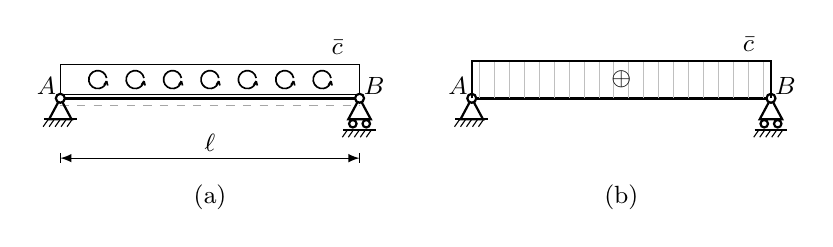
\begin{tikzpicture}[
					scale=0.95,
					>=latex,
					trave/.style={line width=1pt},
					carico/.style={black, line width=0.6pt},
					forza/.style={black, line width=1pt},
					diagT/.style={black, line width=0.8pt},
					hatch/.style={gray!50, line width=0.3pt},
					quota/.style={black, line width=0.4pt},
					fibre/.style={gray!70, line width=0.3pt},
					]
					
					% ── Parametri dei vincoli (convenzione C06/C07) ──
					\def\tw{0.15}    \def\thR{0.28}   \def\rn{0.06}
					\def\rw{0.05}    \def\bw{0.09}    \def\gw{0.22}
					\def\hh{0.10}
					
					% ── Geometria del problema ──
					\def\Lell{4}                            % lunghezza trave ℓ
					\pgfmathsetmacro{\xA}{0}
					\pgfmathsetmacro{\xMid}{0.5*\Lell}      % mezzeria
					\def\yqi{-0.80}                         % y delle quote sotto la trave
					\def\ylab{-3.30}                        % y delle etichette di pannello
					
					% ── Parametri del riquadro delle coppie distribuite ──
					\def\pgap{0.05}                         % gap fra trave e base del riquadro
					\def\php{0.40}                          % altezza del riquadro
					\pgfmathsetmacro{\pBase}{\pgap}         % base del riquadro: y = 0.05
					\pgfmathsetmacro{\pTop}{\pgap+\php}     % cima del riquadro: y = 0.45
					\pgfmathsetmacro{\pMid}{\pgap+0.5*\php} % centro del riquadro: y = 0.25
					\def\rCoppia{0.12}                      % raggio del singolo simbolo "coppia"
					
					% =========================================================
					% PANNELLO (a) — Schema statico
					% =========================================================
					\begin{scope}[xshift=0cm]
						
						% ── Trave ──
						\draw[trave] (0,0) -- (\Lell,0);
						
						% ── Fibra inferiore (tratteggio sotto la trave) ──
						\draw[fibre, dashed] (0, -0.1) -- (\Lell, -0.1);
						
						% ── Cerniera in A ──
						\draw[thick] (0,0) -- (-\tw,-\thR) -- (\tw,-\thR) -- cycle;
						\draw[thick] (-\gw,-\thR) -- (\gw,-\thR);
						\foreach \x in {-0.16,-0.08,0,0.08,0.16}
						\draw[thin] (\x,-\thR) -- ++(-0.07,-\hh);
						
						% ── Carrello verticale in B ──
						\draw[thick] (\Lell,0) -- (\Lell-\tw,-\thR) -- (\Lell+\tw,-\thR) -- cycle;
						\draw[thick] (\Lell-\bw,-\thR-\rw-0.01) circle (\rw);
						\draw[thick] (\Lell+\bw,-\thR-\rw-0.01) circle (\rw);
						\draw[thick] (\Lell-\gw,-\thR-2*\rw-0.04) -- (\Lell+\gw,-\thR-2*\rw-0.04);
						\foreach \x in {-0.16,-0.08,0,0.08,0.16}
						\draw[thin] (\Lell+\x,-\thR-2*\rw-0.04) -- ++(-0.07,-\hh);
						
						% ── Anellini bianchi sui perni ──
						\draw[thick, fill=white] (0,0) circle (\rn);
						\draw[thick, fill=white] (\Lell,0) circle (\rn);
						
						% ── Etichette A, B ──
						\node[above left=-2pt,  font=\small] at (0,0)      {$A$};
						\node[above right=-2pt, font=\small] at (\Lell,0)  {$B$};
						
						% ── Riquadro delle coppie distribuite ──
						\draw[carico] (0,\pBase) -- (\Lell,\pBase);
						\draw[carico] (0,\pTop)  -- (\Lell,\pTop);
						\draw[carico] (0,\pBase) -- (0,\pTop);
						\draw[carico] (\Lell,\pBase) -- (\Lell,\pTop);
						
						
						% ── Sette simboli "coppia antioraria" equispaziati ──
						\def\Lwing{0.06}    % lunghezza dell'ala della freccia
						\foreach \xs in {0.50, 1.00, 1.50, 2.00, 2.50, 3.00, 3.50} {
							% Arco quasi chiuso (340°, apertura 20°) — senza freccia automatica
							\draw[carico]
							({\xs+\rCoppia*cos(10)}, {\pMid+\rCoppia*sin(10)})
							arc[start angle=10, end angle=350, radius=\rCoppia];
							
							% Punta della freccia disegnata a due tratti, all'estremità a θ=350°
							\pgfmathsetmacro{\tipx}{\xs + \rCoppia*cos(350)}
							\pgfmathsetmacro{\tipy}{\pMid + \rCoppia*sin(350)}
							\draw[carico] (\tipx, \tipy)
							-- ({\tipx + \Lwing*cos(235)}, {\tipy + \Lwing*sin(235)});
							\draw[carico] (\tipx, \tipy)
							-- ({\tipx + \Lwing*cos(285)}, {\tipy + \Lwing*sin(285)});
						}
						
						% Etichetta c̄ sopra il riquadro, a destra
						\node[above, font=\small] at (\Lell-0.30, \pTop) {$\bar{c}$};
						
						% ── Quota ℓ sotto la trave ──
						\draw[<->, quota] (0,\yqi) -- (\Lell,\yqi);
						\draw[quota] (0,\yqi+0.07)     -- (0,\yqi-0.07);
						\draw[quota] (\Lell,\yqi+0.07) -- (\Lell,\yqi-0.07);
						\node[above, font=\small] at (\xMid, \yqi-0.04) {$\ell$};
						
						% Etichetta pannello (a)
						\node[font=\small] at (0.5*\Lell, 0.4*\ylab) {(a)};
						
					\end{scope}
					
					% =========================================================
					% PANNELLO (b) — Diagramma di T(z)
					% =========================================================
					\begin{scope}[xshift=5.5cm]
						
						% ── Trave (clone) ──
						\draw[trave] (0,0) -- (\Lell,0);
						
						% ── Vincoli (clone) ──
						\draw[thick] (0,0) -- (-\tw,-\thR) -- (\tw,-\thR) -- cycle;
						\draw[thick] (-\gw,-\thR) -- (\gw,-\thR);
						\foreach \x in {-0.16,-0.08,0,0.08,0.16}
						\draw[thin] (\x,-\thR) -- ++(-0.07,-\hh);
						\draw[thick] (\Lell,0) -- (\Lell-\tw,-\thR) -- (\Lell+\tw,-\thR) -- cycle;
						\draw[thick] (\Lell-\bw,-\thR-\rw-0.01) circle (\rw);
						\draw[thick] (\Lell+\bw,-\thR-\rw-0.01) circle (\rw);
						\draw[thick] (\Lell-\gw,-\thR-2*\rw-0.04) -- (\Lell+\gw,-\thR-2*\rw-0.04);
						\foreach \x in {-0.16,-0.08,0,0.08,0.16}
						\draw[thin] (\Lell+\x,-\thR-2*\rw-0.04) -- ++(-0.07,-\hh);
						\draw[thick, fill=white] (0,0) circle (\rn);
						\draw[thick, fill=white] (\Lell,0) circle (\rn);
						
						% ── Etichette A, B ──
						\node[above left=-2pt,  font=\small] at (0,0)      {$A$};
						\node[above right=-2pt, font=\small] at (\Lell,0)  {$B$};
						
						% ── Diagramma T(z) ──
						\def\sT{0.50}
						\pgfmathsetmacro{\Tval}{\sT}        % T(z) = +c̄ → +0.50
						
						% Hatching verticale uniforme su tutta la trave
						\foreach \x in {0.10, 0.30, ..., 3.90} {
							\draw[hatch] (\x, 0) -- (\x, \Tval);
						}
						
						% Bordo del diagramma — rettangolo
						\draw[diagT]
						(0, 0) -- (0, \Tval)             % verticale in A
						-- (\Lell, \Tval)                % uniforme su tutta la trave
						-- (\Lell, 0);                   % verticale di chiusura in B
						
						% Segno cerchiato al centro del rettangolo
						\node[font=\small] at (\xMid, {0.5*\Tval})
						{$\boldsymbol{\oplus}$};
						
						% Etichetta del valore c sopra il rettangolo, vicino al bordo destro
						\node[above, font=\small] at (\Lell-0.30, \Tval) {$\bar{c}$};
						
						% Etichetta pannello (b)
						\node[font=\small] at (0.5*\Lell, 0.4*\ylab) {(b)};
						
					\end{scope}
					
				\end{tikzpicture}
				%}
			\caption{Trave appoggiata con coppie antiorarie uniformemente
				distribuite di intensità $\bar{c}$ su tutta la lunghezza:
				(a)~schema strutturale;
				(b)~diagramma del taglio $T(z)$, uniforme pari a $\bar{c}$
				su tutta la trave.
				Il momento flettente è identicamente nullo, $M(z) \equiv 0$,
				e non è riportato in figura: le coppie distribuite
				compensano esattamente il contributo del taglio
				($M' = T - c = 0$).}
			\label{fig:stat_trasv_iso_06}
		\end{figure}
